We begin by performing a very simple screening of the available potentials using 0~K potential energy calculations.
The Fe-Al phase diagram for the relevant ideal phases in shown in Fig.~\ref{fig:0K_phases}.
Here we can already see that the potentials of Farkas \etal~\cite{farkas2020model} and Jelinek \etal~\cite{jelinek2012modified} both fail to provide clear BCC stability.
This is not shocking as these were both designed for high-entropy alloys, and the former is explicitly targeted towards the FCC phase.
Nonetheless, for the rest of our investigation we can safely focus on the EAM potential of Mendelev \etal~\cite{mendelev2005effect} and the more recent MEAM potential of Lee and Lee \etal~\cite{lee2010modified}.
%
\begin{figure}[h]
    \centering
    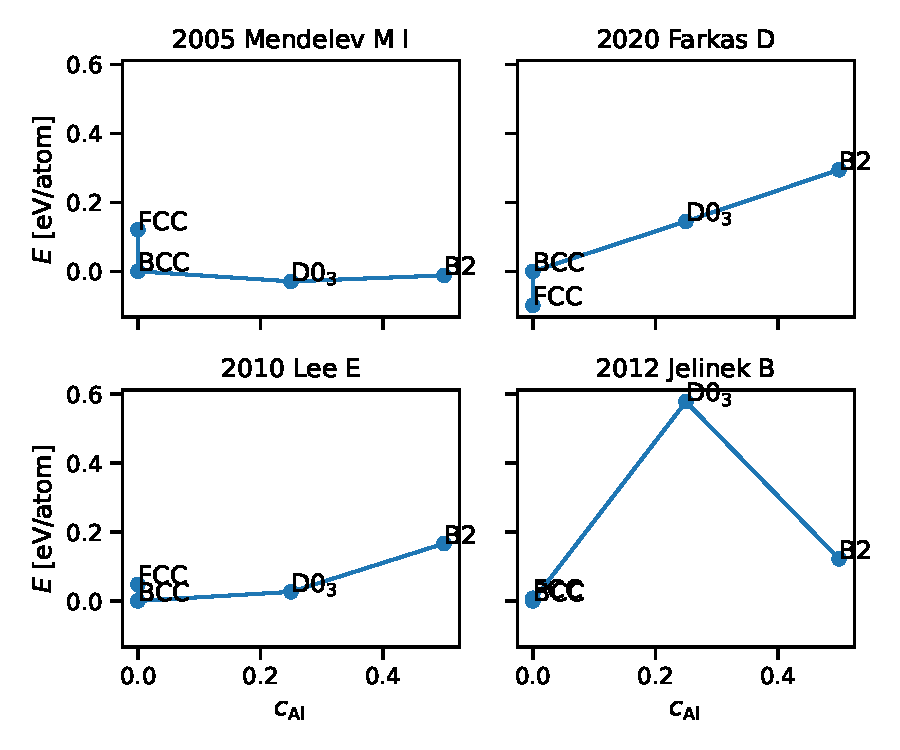
\includegraphics[width=\textwidth]{figures/zerok_phases}
    \caption{0K potential energy/atom for each of the relevant Fe-Al phases up to 50\% Al for several empirical potentials~\cite{mendelev2005effect, lee2010modified, jelinek2012modified, farkas2020model}.}
    \label{fig:0K_phases}
\end{figure}

In addition to being BCC stable, we know that the potentials should be dominated by a solid solution at 18\% Al, and that the \DOTHREE phase should also be energetically competitive such that it has the chance of appearing as small SRO clusters.
To this end, we expand the diagram in Fig.~\ref{fig:TODO} contains additional data including information about the random solid solution state at Al concentrations up to the nominal \DOTHREE concentration.
At each concentration ten different random configurations of a $3\times3\times3$ supercell (432) atoms we relaxed at zero pressure, and the final energy averaged over.
The error bars for the solid solution shows the 95\% confidence interval from the sampling (i.e. roughly double the standard deviation).
In addition to the solid solution and normal phases, we also show data for other ordered phases: columnar Al with varying inter-columnar spacing (similar to pin-like \BTWO precipitates) and planar Al wiht varying inter-planar spacing.
Representatives of all of these are visualized in Fig.~\ref{fig:TODO}.

In addition to the 0~K potential energy, for the solid solution data the ideal entropy of mixing was included at both the experimental annealing temperatures.
This demonstrates the increasing benefit to the \emph{free} energy for the system to occupy a disordered state.
In principle the entropy of mixing is also relevant for the other phases -- even our SRO clusters may contain chemical antisites and do not need to \emph{perfectly} conform to the reference ordering -- but at this stage they are omitted, as is vibrational entropy for all phases.
Even with these simplifications, we can already draw important conclusions: first, the Mendelev potential will never display \DOTHREE SRO at 18\% Al.
Constructing a parallel tangent line between the minima of the phases, we can expect the system is likely to form either a composition of solid solution and the layered structure, or simply form into ordered layers.
The potential energy of this layered structure sits so far below the \DOTHREE phase that we should never expect to see \DOTHREE form in any significant fraction.
Second, for the Lee potential, a similar Gibbs-tie-line analysis shows that decomposition into solid solution and \DOTHREE \emph{is} possible, but may only occur at higher temperatures than we expect from experiment.
This potential seems to have an unphysically low solubility of Al in bulk BCC Fe.
